\section{Versuchsafbau}
    \subsection*{Röntgenografische Methode}
    Für die röntgenografische Methode steht im Versuch ein Röntgendiffraktometer zur Verfügung.
    Dabei sitzt die Probe in der Mitte eines Detektors welcher Röntegenstrahlung detektieren kann.
    Die Probe wird dann mit einer von einer Röntgenröhre erzeugter Röntgenstrahlung bestrahlt, welche
    an den Gitterebenen der Probe reflektiert und auf dem Detektorschirm abgebildet wird.
    \begin{figure}[H]
        \centering
        \begin{subfigure}{.5\textwidth}
        \centering
        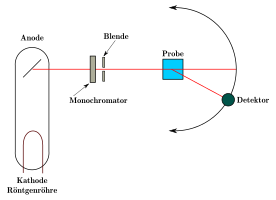
\includegraphics[width=.8\linewidth]{images/diffraktometer.png}
        \caption{}
        \label{fig:sub1}
        \end{subfigure}%
        \begin{subfigure}{.5\textwidth}
        \centering
        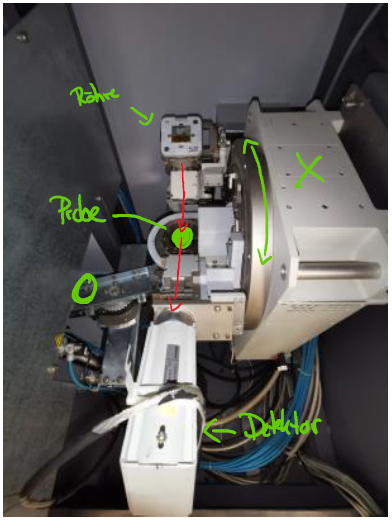
\includegraphics[width=.6\linewidth]{images/diffraktometer_pic.png}
        \caption{}
        \label{fig:sub2}
        \end{subfigure}
        \caption{a) Schematischer Aufbau eines Röntgendiffraktometers b) Foto des Röntgendiffraktometers}
        \label{fig:test}
    \end{figure}
    \subsection*{Resistives Verfahren}
    Bei dem resistiven Verfahren müssen zunächst die Proben auf einem Stab fixiert werden, anschließen werden
    an der Probe die Leitungen mit Silberpaste leitend befestigt. Anschließend wird der Stab mit der fixierten
    Probe an einem Schrittmotor befestigt um die Probe in einen Heliumbehälter auf variable Höhen zu bewegen.
    Beim befestigen der Leiter auf der Probe ist dabei zu achten, dass der Abstand zwischen den Kontakten möglichst
    homogen ist und, dass die Kontakte richtig verschaltet sind um die Messung nicht durch die Innenwiderstände
    der Messelektronik zu beeinflussen. Dazu nutzt mann folgenden schaltplan
    \begin{figure}[H]
        \centering
        \begin{subfigure}{.5\textwidth}
        \centering
        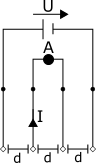
\includegraphics[width=.4\linewidth]{images/schaltplan.png}
        \caption{}
        \label{fig:sub11}
        \end{subfigure}%
        \begin{subfigure}{.5\textwidth}
        \centering
        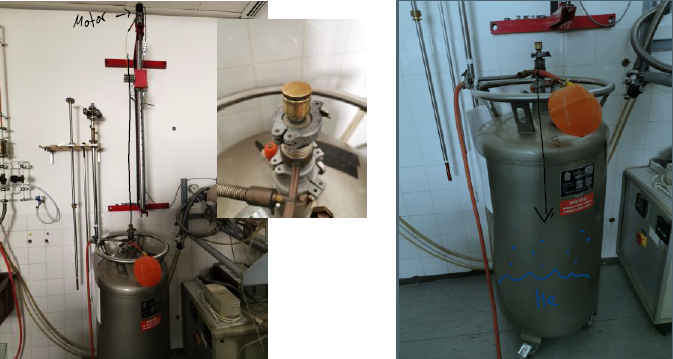
\includegraphics[width=.8\linewidth]{images/aufbaures.png}
        \caption{}
        \label{fig:sub22}
        \end{subfigure} 
        \caption{a) Beschaltung des 4-Punkt messstabes b) Bild des Messaufbaus mit Motor, Proben messtab und Heliumbehälter}
        \label{fig:test1}
    \end{figure}

